\documentclass[11pt]{article}
\usepackage[margin=1in]{geometry}
\usepackage{booktabs}
\usepackage{graphicx}
\usepackage{float}
\begin{document}
\section*{Supplementary Step 11 Visualization Report}
\subsection*{Overview}
\begin{tabular}{p{0.42\linewidth}p{0.50\linewidth}}
\toprule
Metric & Value\\
\midrule
Included participant-sessions & 36\\
Included questions & 30\\
Included trials & 1075\\
Primary robust SE type & Two-way cluster (participant + question)\\
Primary continuous p-value & 0.303503\\
Binary benchmark p-value & 0.209749\\
Quadratic linear-term p-value & 0.188168\\
Quadratic squared-term p-value & 0.218468\\
Threshold-strength p-value & 0.504510\\
Back ROI benchmark p-value & 0.404042\\
Fixed-window benchmark p-value & 0.271618\\
No-override p-value & 0.481741\\
Binary cutoff used & 0.50\\
Questions below / above cutoff & 15 / 15\\
\bottomrule
\end{tabular}
\paragraph{Interpretation note.} In the participant-fixed-effects regression using the continuous abstractness score, the association between abstractness level and left frontal ROI HbO response was not statistically significant (beta=1.311e-08, SE=1.251e-08, p=0.303503, 95\% CI [-1.249e-08, 3.870e-08]). This suggests that replacing the binary label with a continuous abstractness measure does not by itself yield robust evidence for a frontal abstractness effect in the current dataset. The binary benchmark remained non-significant (p=0.209749), the fixed-window continuous benchmark remained non-significant (p=0.271618), and the no-override continuous model remained non-significant (p=0.481741).
\paragraph{Correlation note.} Score-diagnostic correlations were: Total word count: r=0.040, p=0.832348; Sentence count: r=-0.011, p=0.953914; Average sentence length: r=0.035, p=0.855832; ENEM item correctness: r=0.400, p=0.028305; Mean response time: r=0.010, p=0.956933.
\subsection*{Core Step 11 Figures}
\begin{figure}[H]
\centering
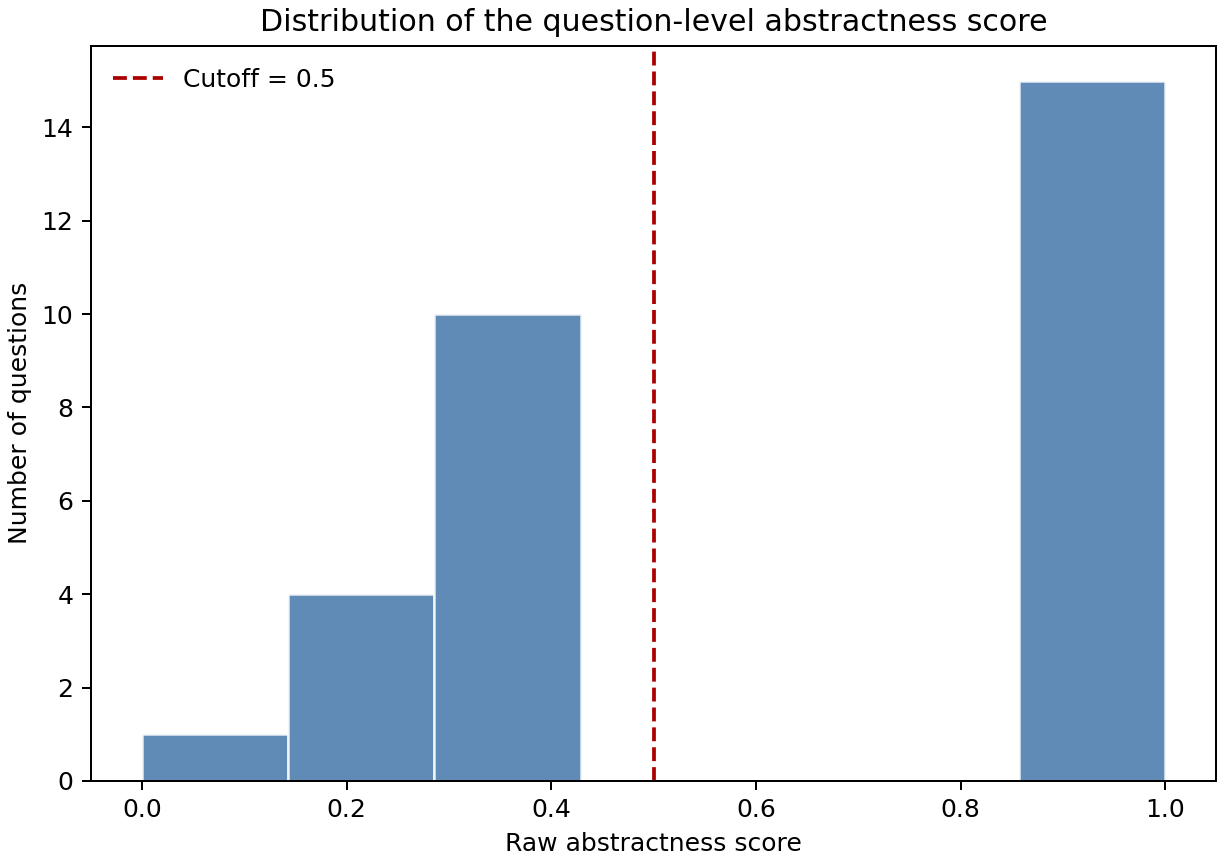
\includegraphics[width=0.48\linewidth]{../../figures/step11/score_histogram.png}
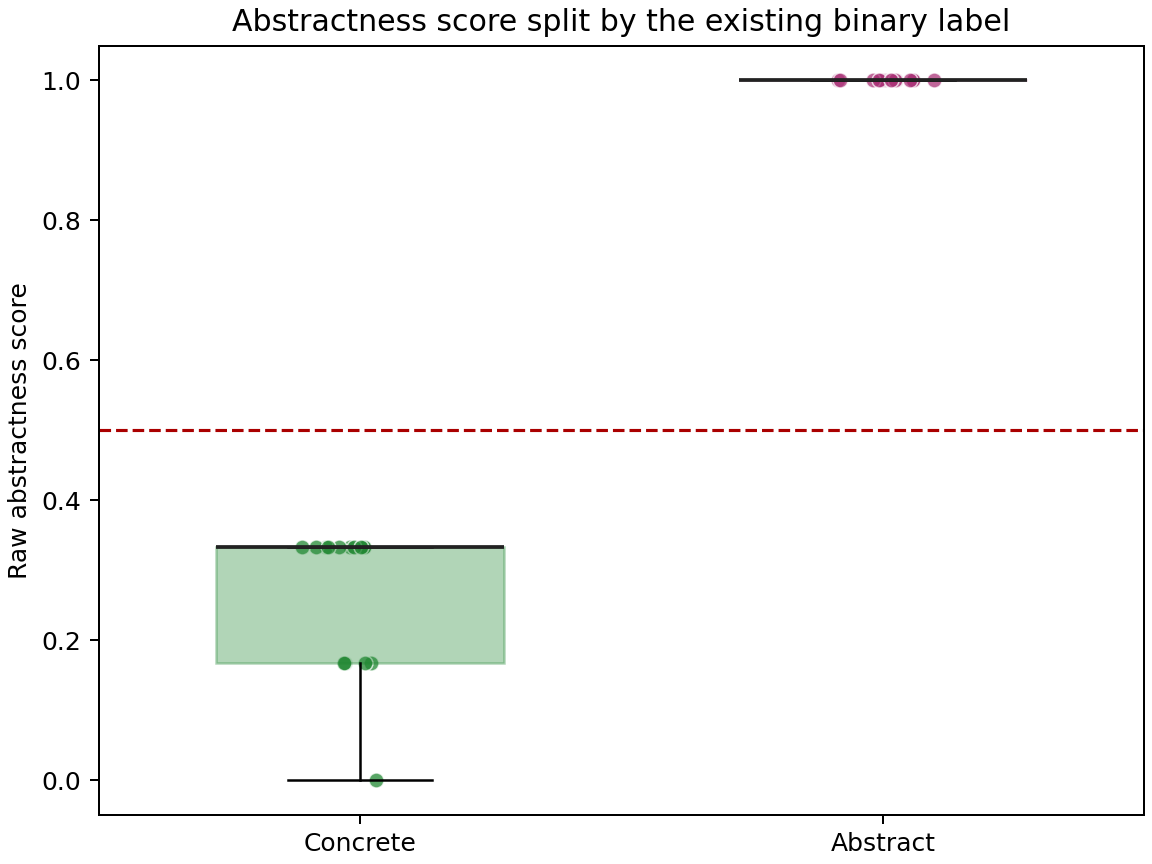
\includegraphics[width=0.48\linewidth]{../../figures/step11/score_by_binary_label.png}
\caption{Distribution of the raw abstractness score and its split by the existing binary label.}
\end{figure}
\begin{figure}[H]
\centering
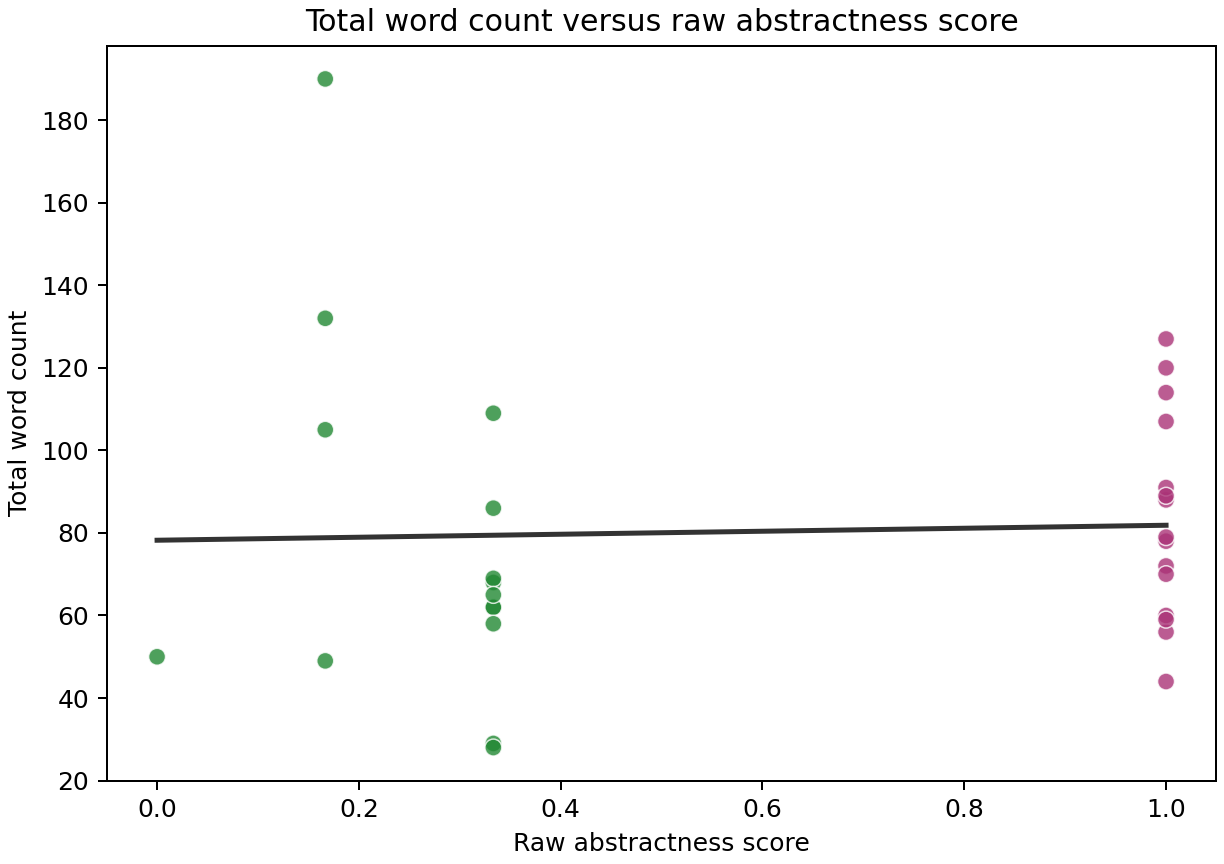
\includegraphics[width=0.48\linewidth]{../../figures/step11/score_vs_wordcount.png}
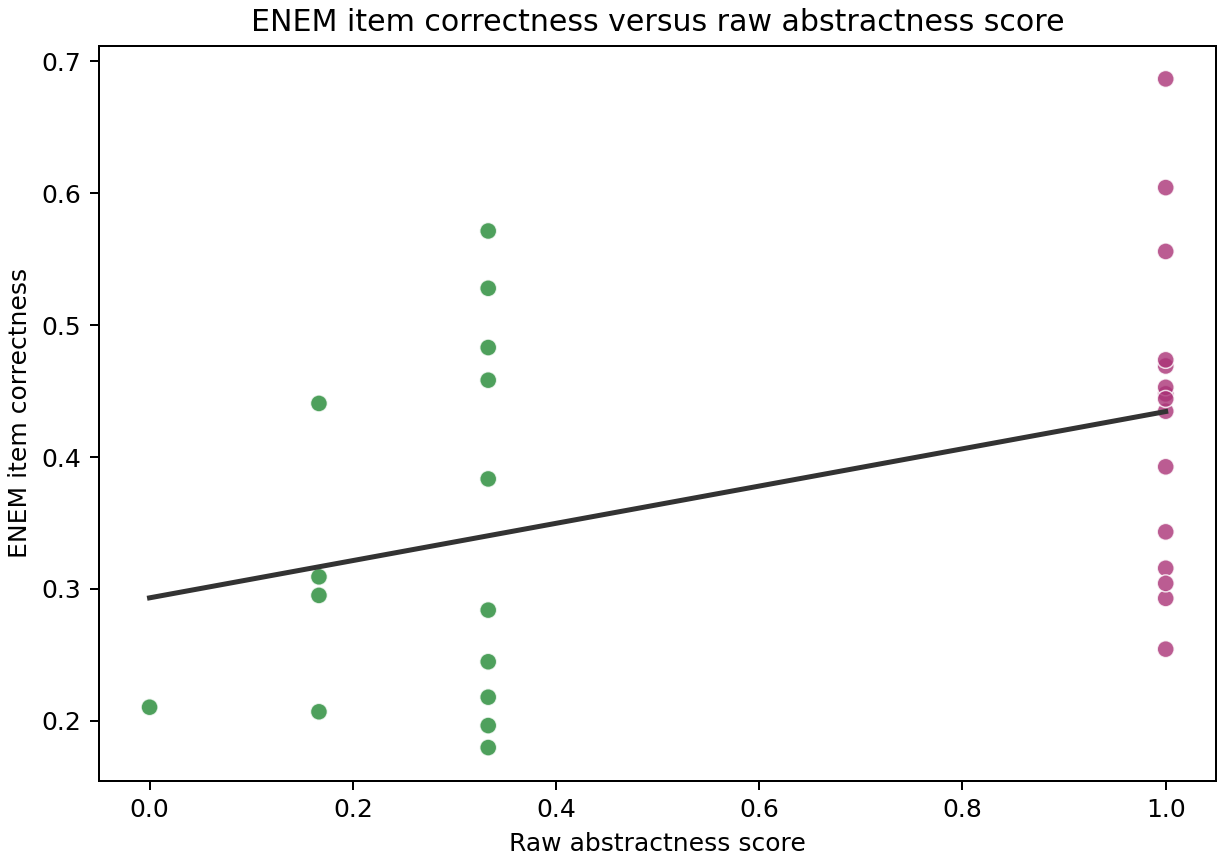
\includegraphics[width=0.48\linewidth]{../../figures/step11/score_vs_correctness.png}
\caption{Abstractness score against total word count and ENEM item correctness.}
\end{figure}
\begin{figure}[H]
\centering
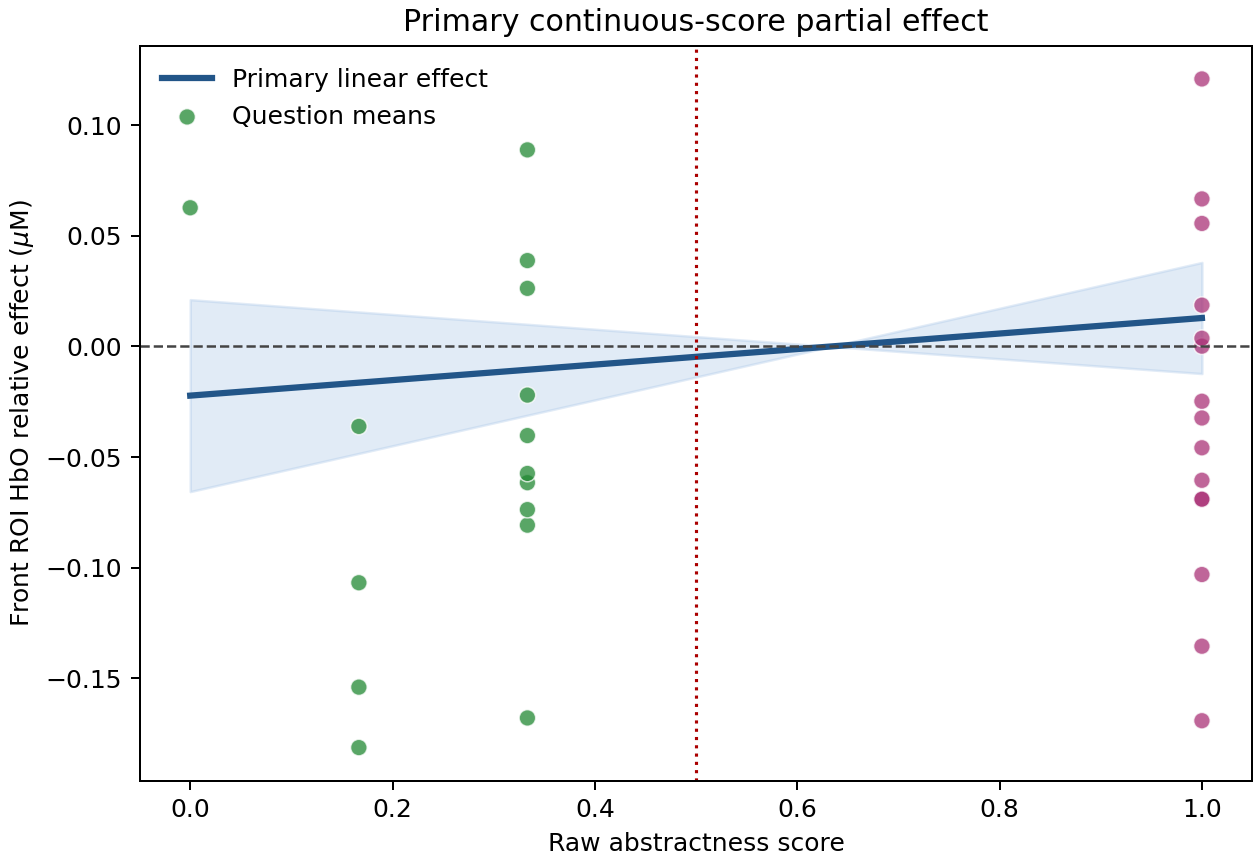
\includegraphics[width=0.48\linewidth]{../../figures/step11/continuous_partial_effect_plot.png}
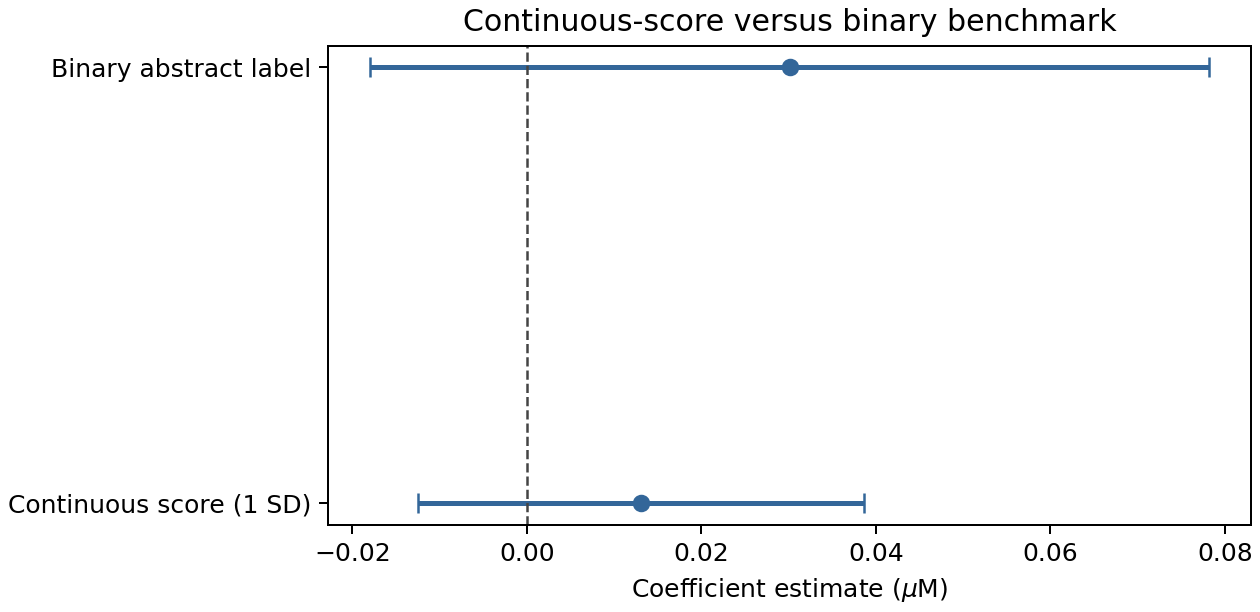
\includegraphics[width=0.48\linewidth]{../../figures/step11/continuous_vs_binary_benchmark.png}
\caption{Primary continuous-score partial effect and the comparison against the binary benchmark.}
\end{figure}
\begin{figure}[H]
\centering
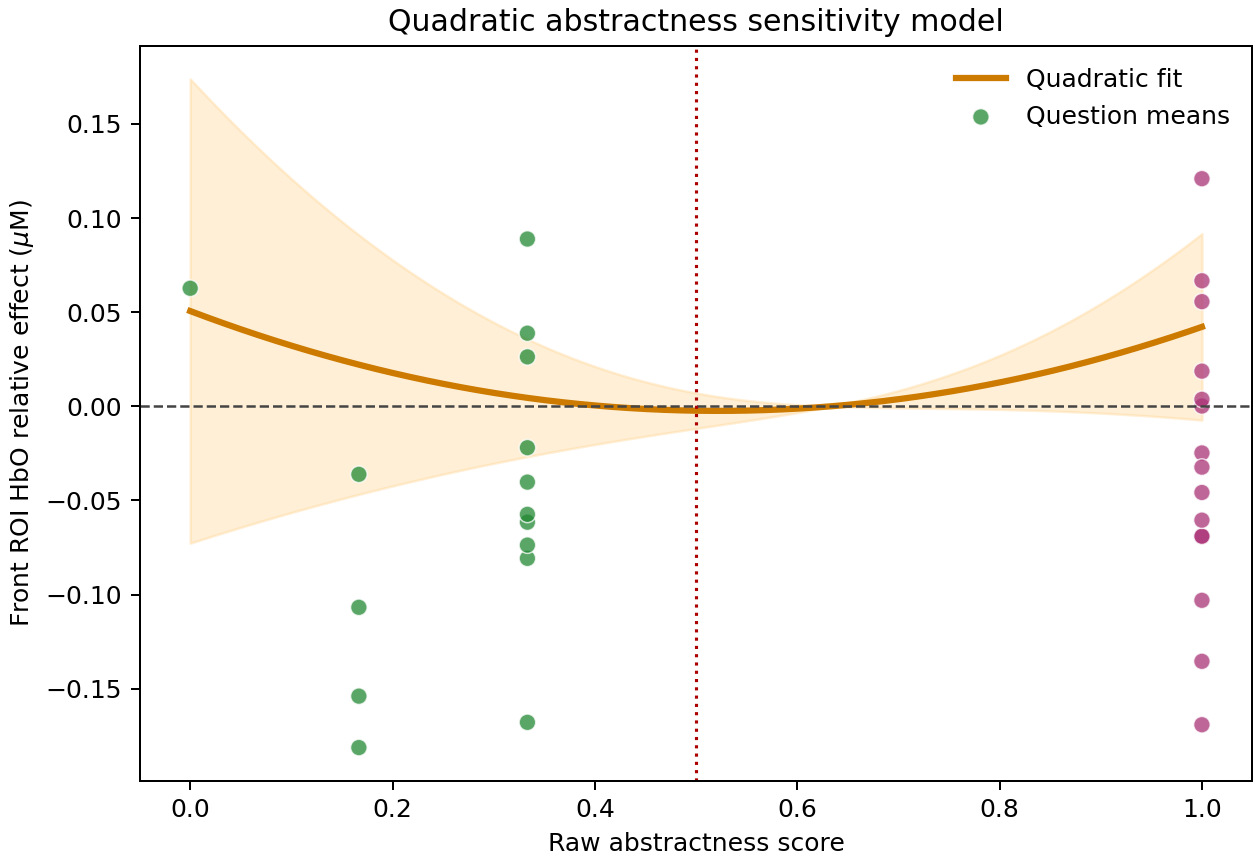
\includegraphics[width=0.48\linewidth]{../../figures/step11/quadratic_effect_plot.png}
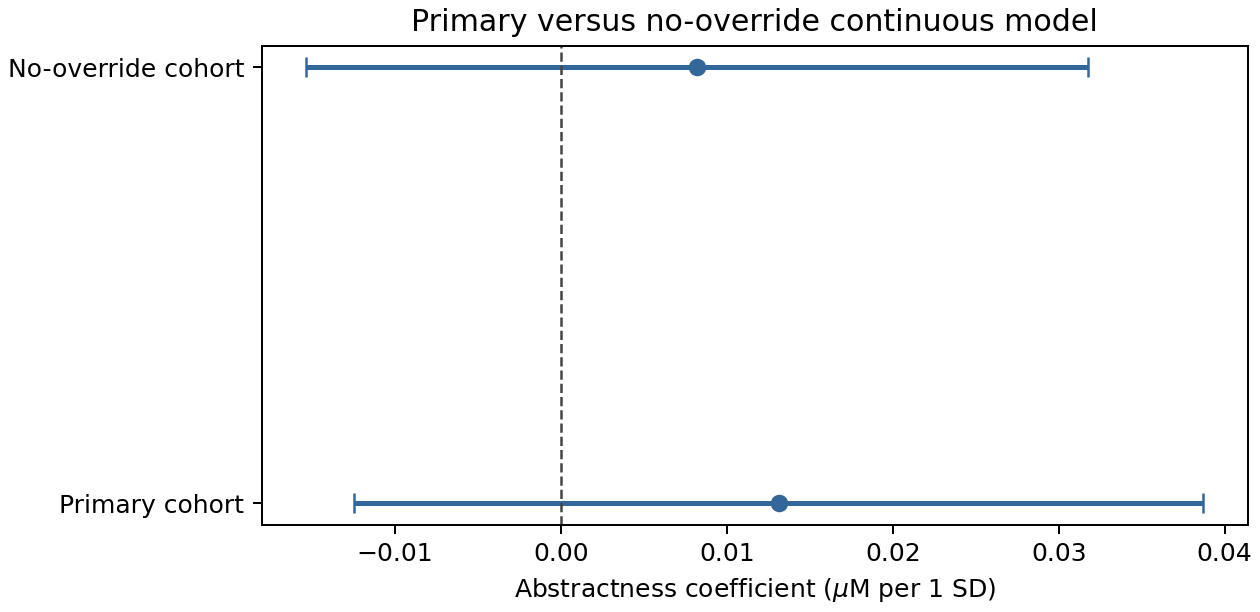
\includegraphics[width=0.48\linewidth]{../../figures/step11/no_override_comparison.png}
\caption{Quadratic sensitivity visualization and the no-override comparison.}
\end{figure}
\begin{figure}[H]
\centering
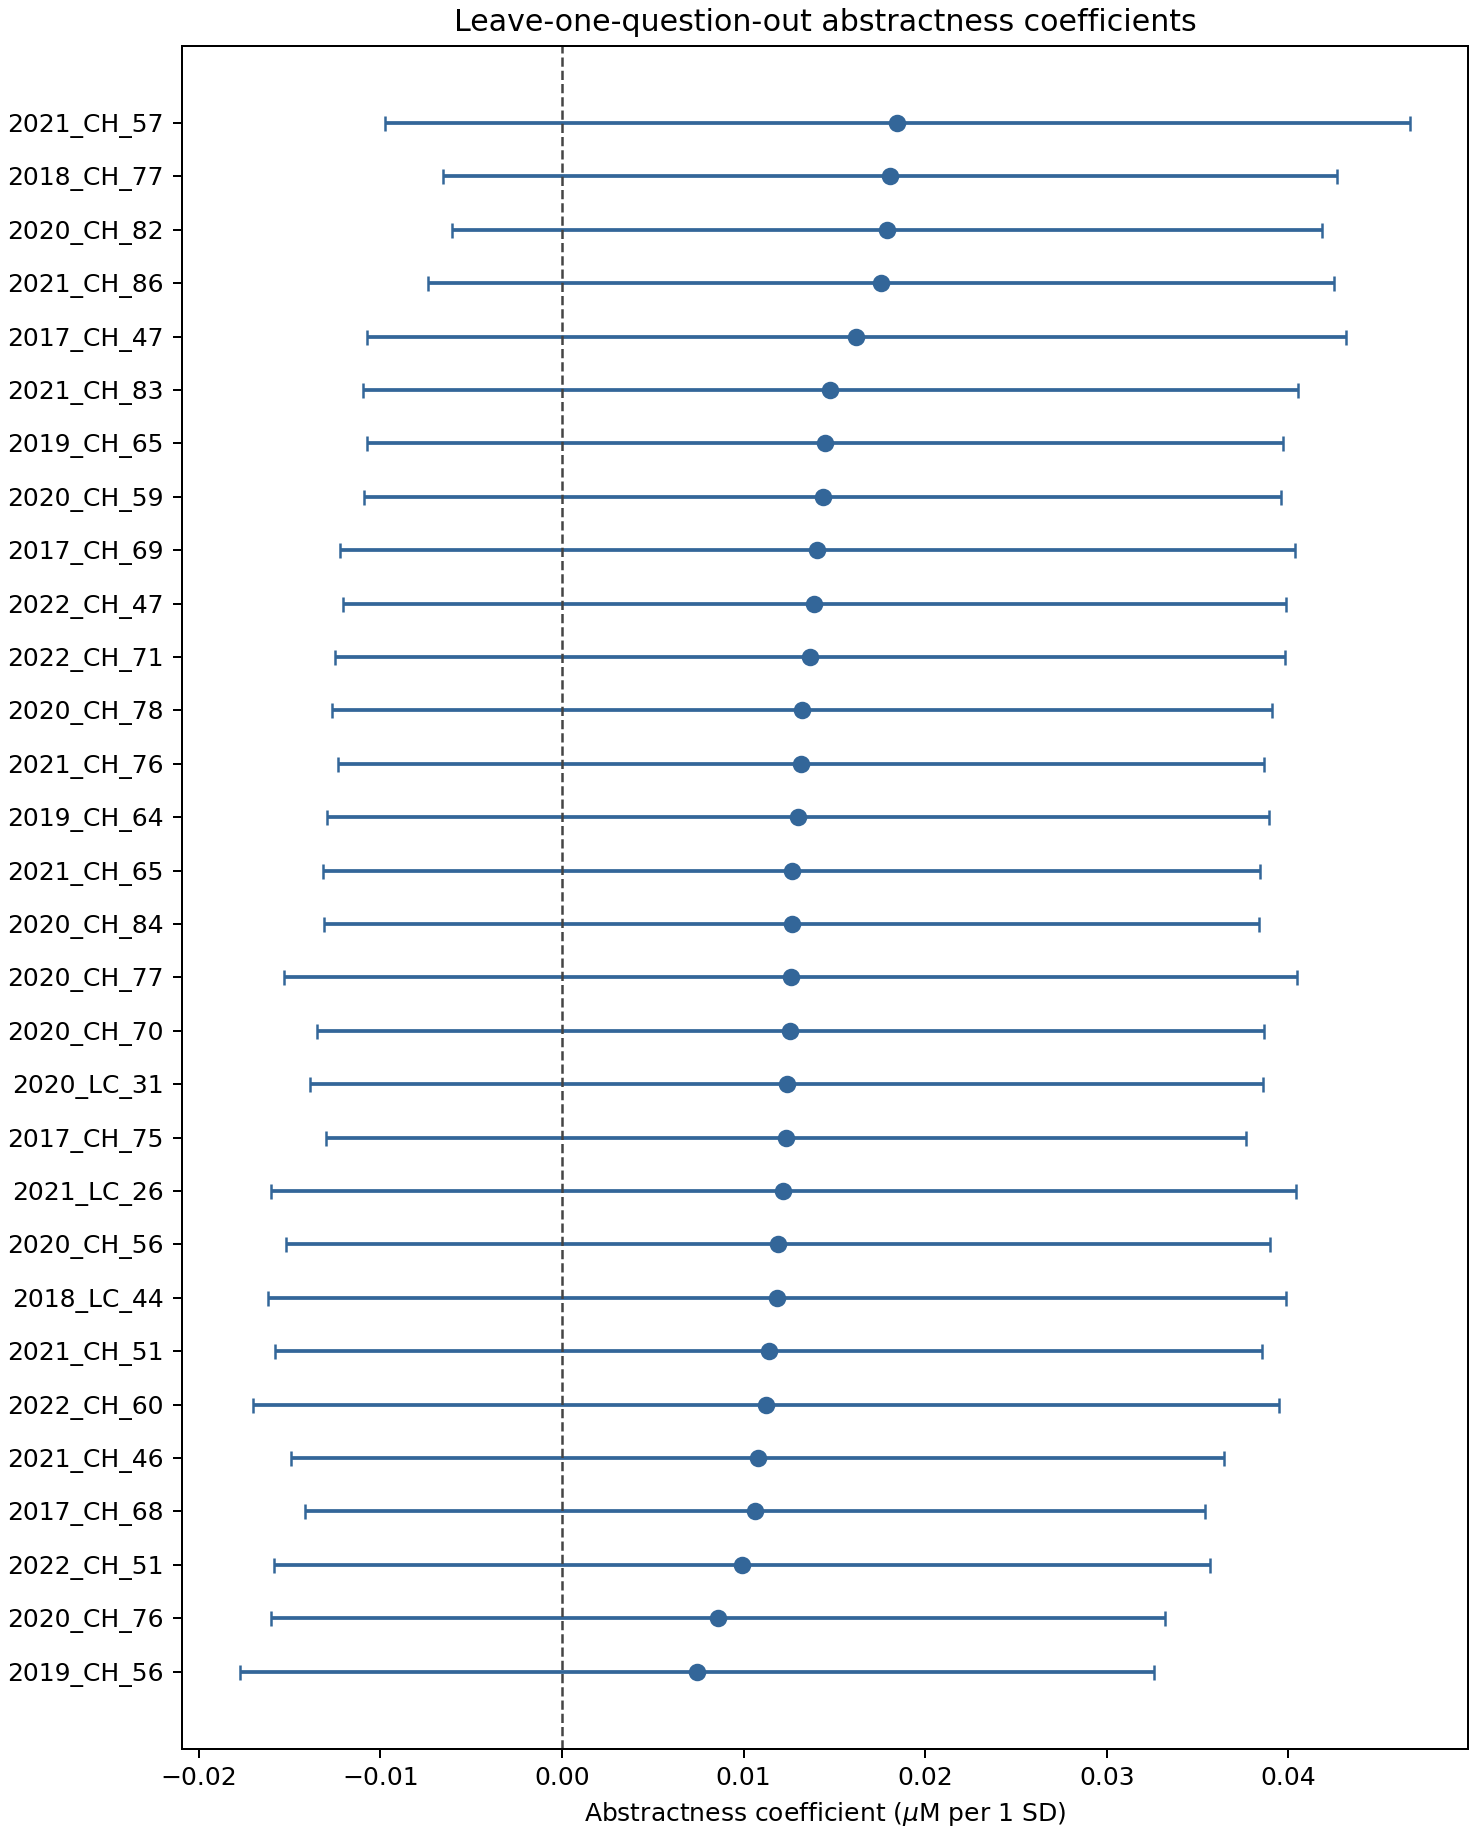
\includegraphics[width=0.82\linewidth]{../../figures/step11/leave_one_question_out_plot.png}
\caption{Leave-one-question-out abstractness coefficients from the main Step~11 run.}
\end{figure}
\subsection*{Additional Step 11 Diagnostics}
\begin{figure}[H]
\centering
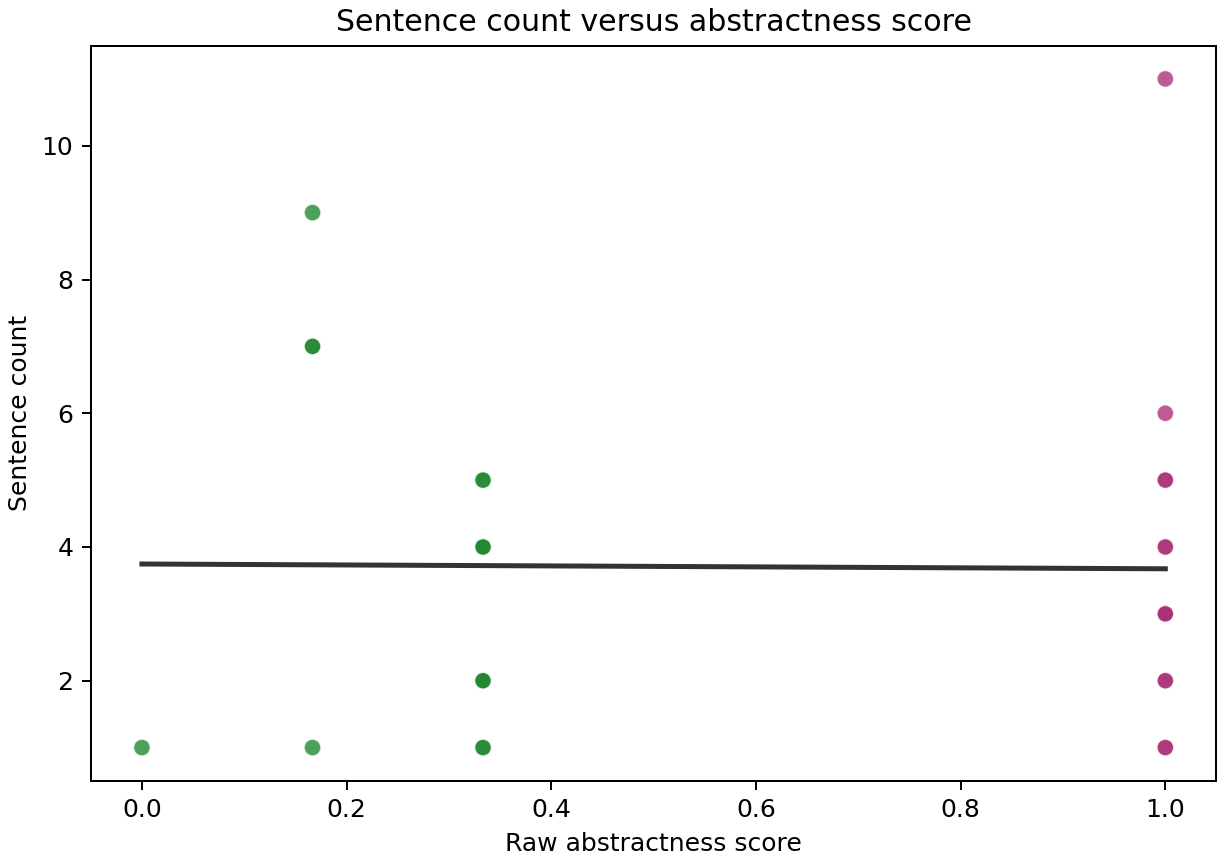
\includegraphics[width=0.32\linewidth]{../../figures/step11_visualization/score_vs_sentence_count.png}
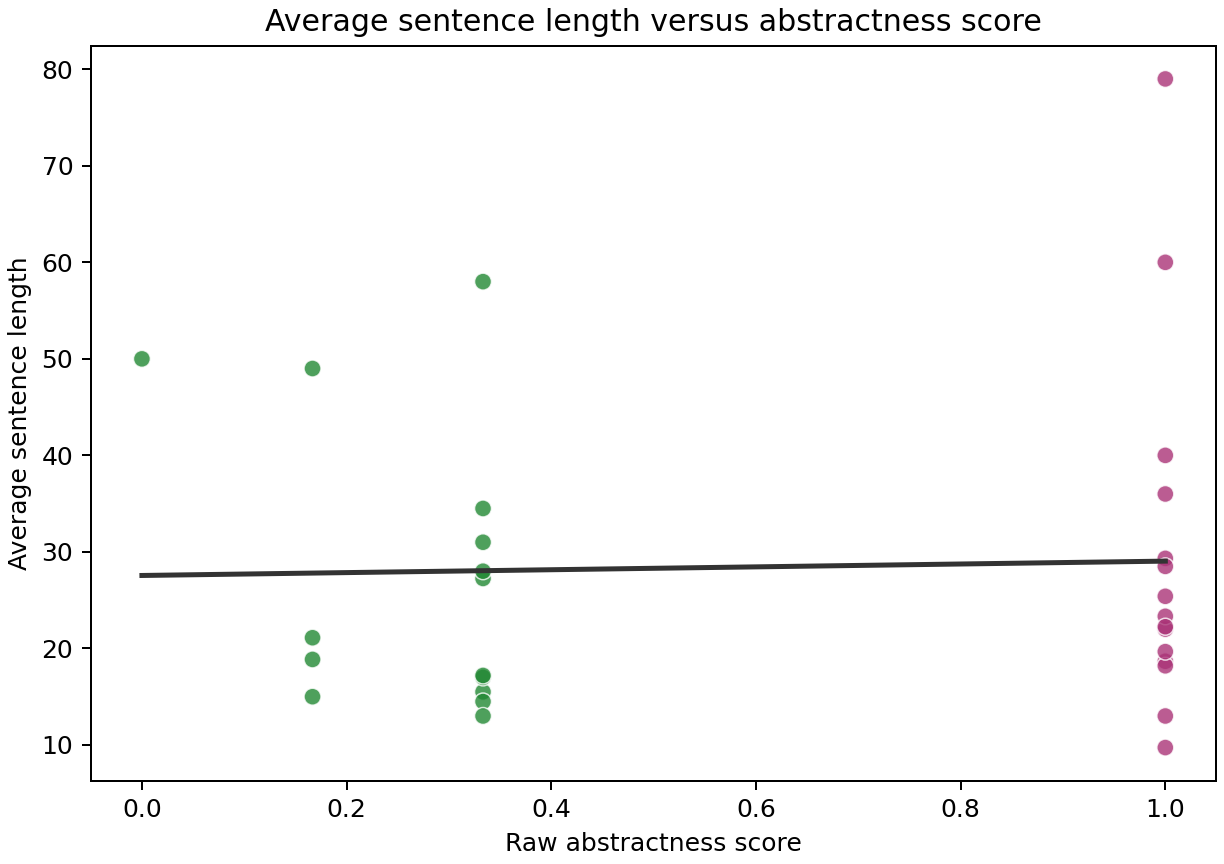
\includegraphics[width=0.32\linewidth]{../../figures/step11_visualization/score_vs_sentence_length.png}
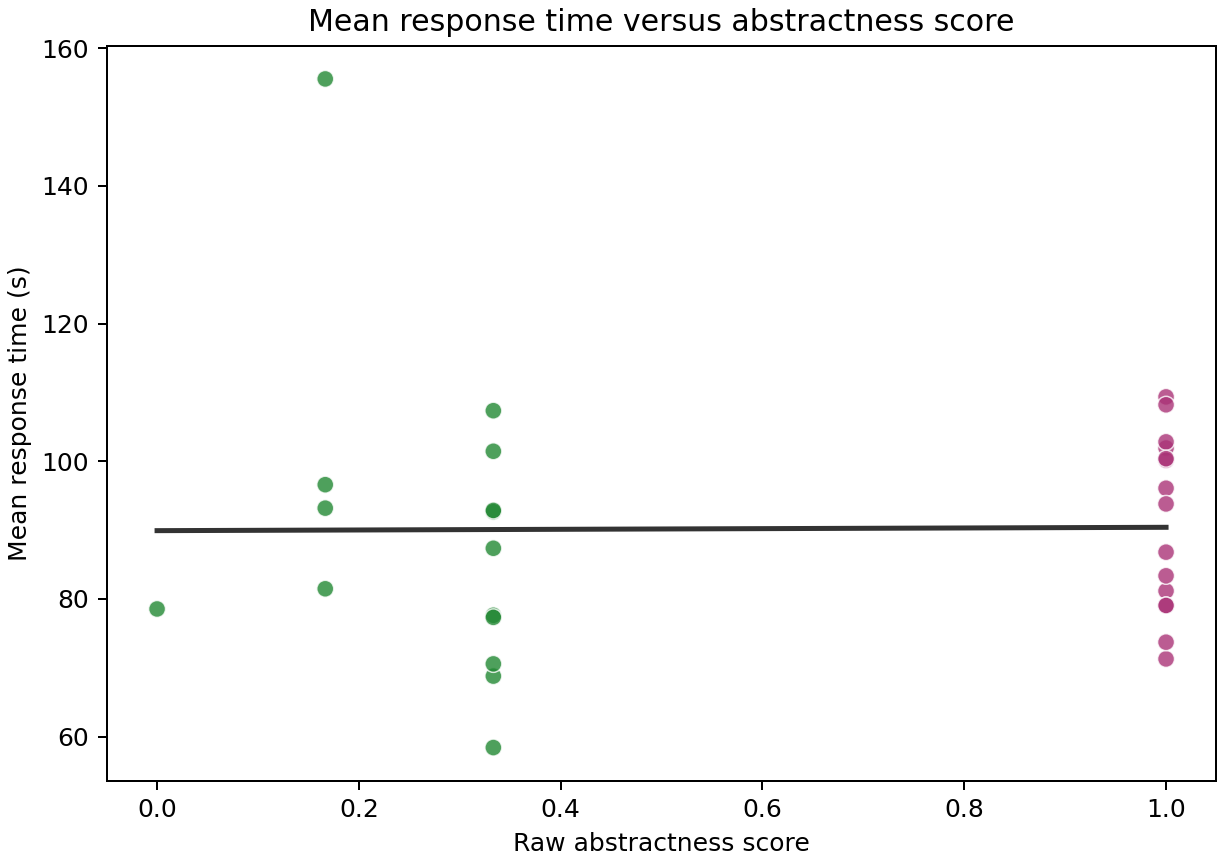
\includegraphics[width=0.32\linewidth]{../../figures/step11_visualization/score_vs_response_time.png}
\caption{Additional score-diagnostic scatter plots for sentence count, sentence length, and mean response time.}
\end{figure}
\begin{figure}[H]
\centering
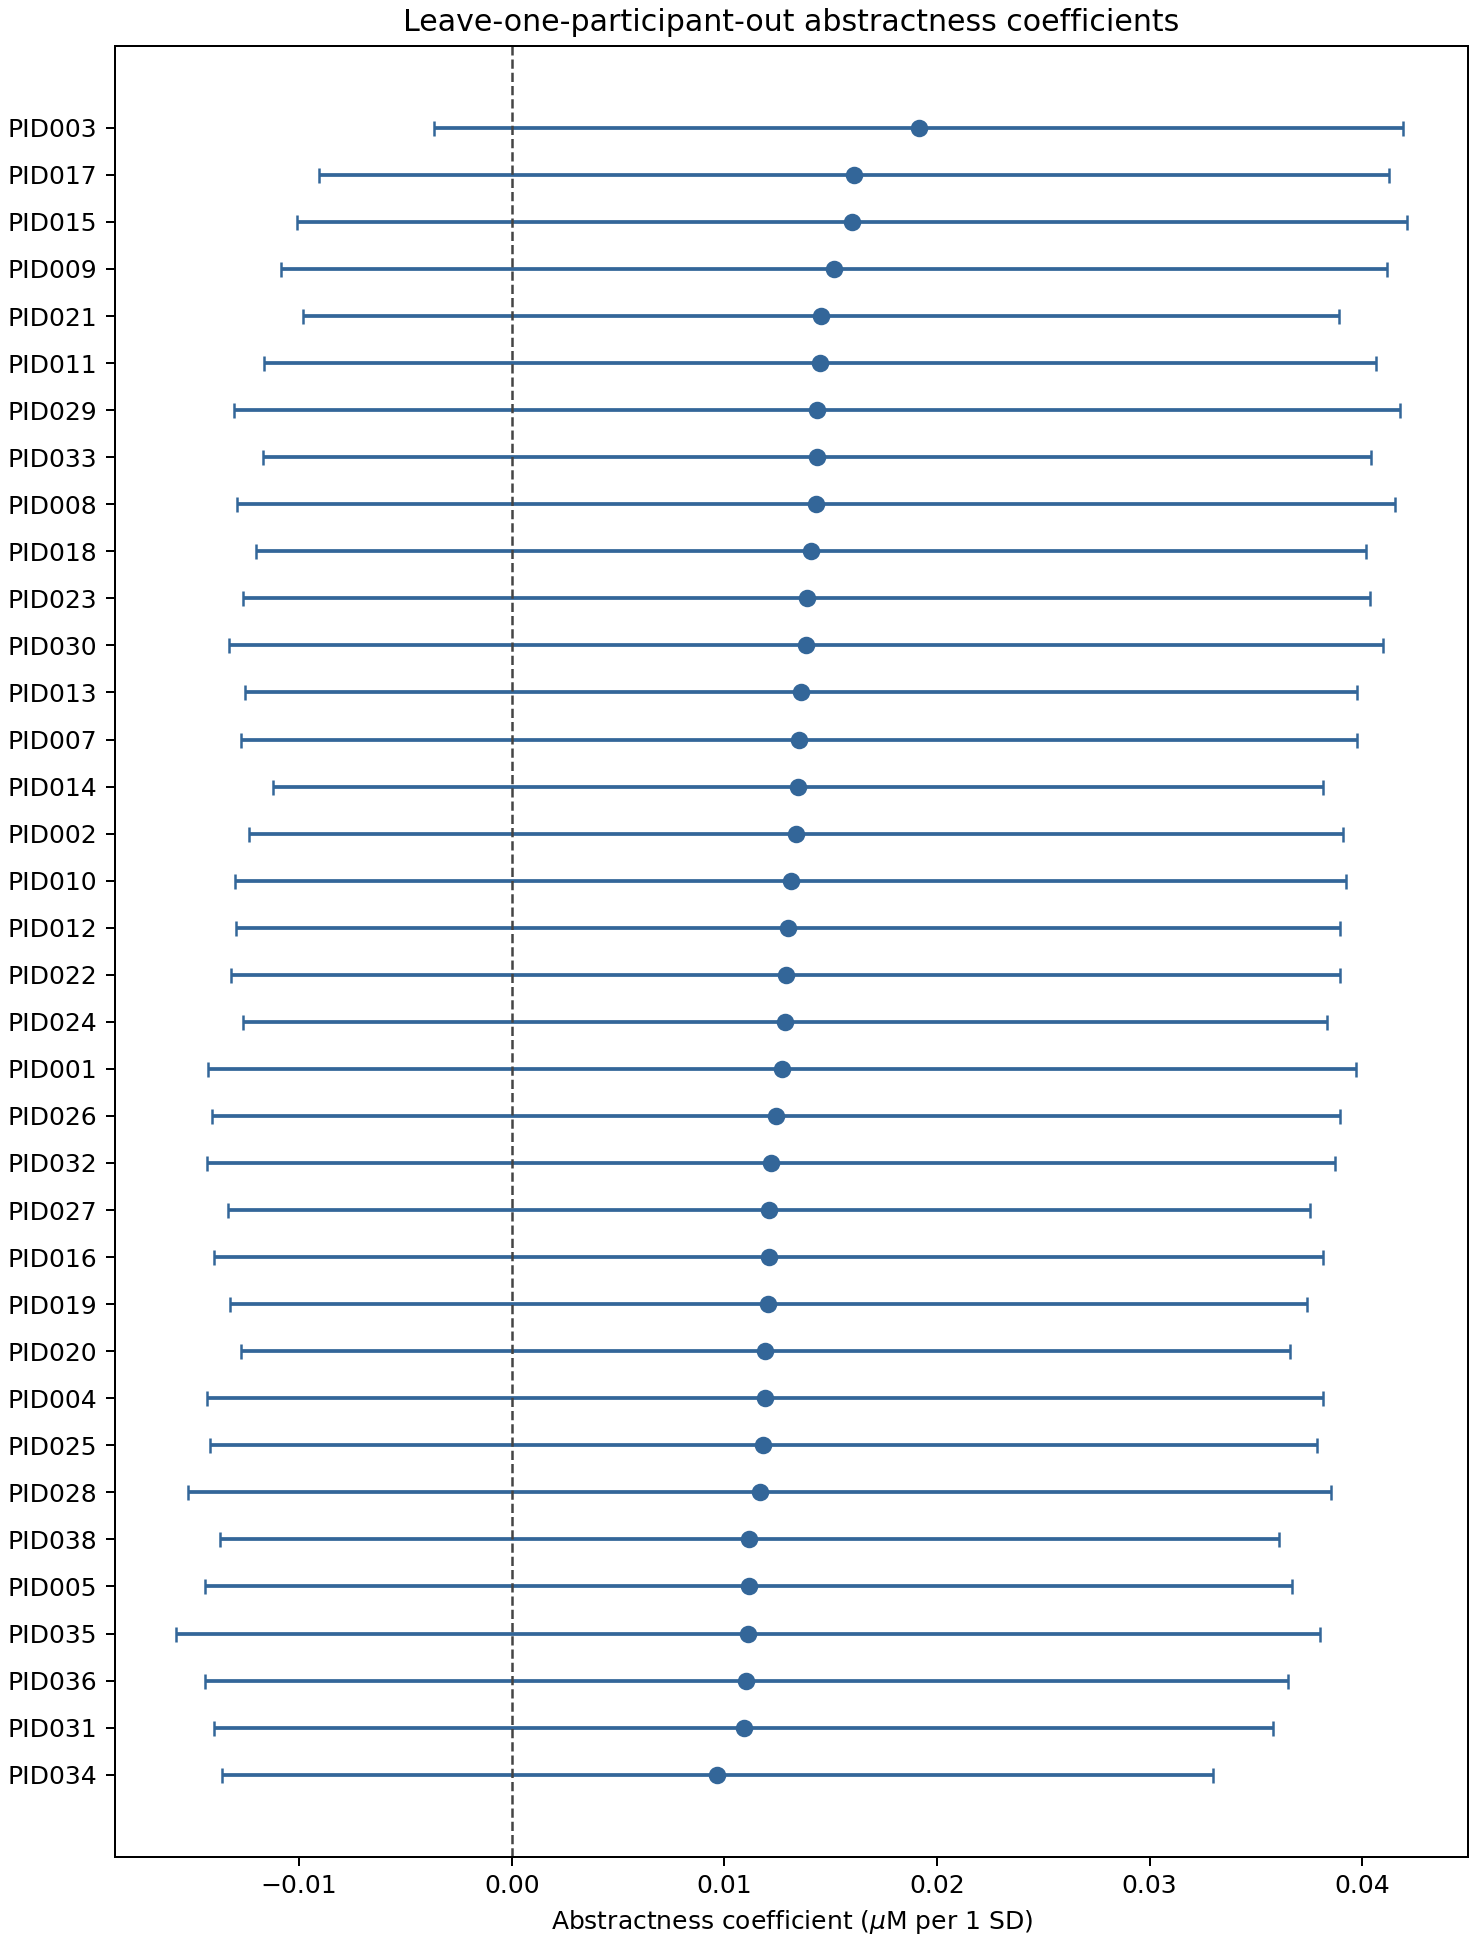
\includegraphics[width=0.48\linewidth]{../../figures/step11_visualization/leave_one_participant_out_plot.png}
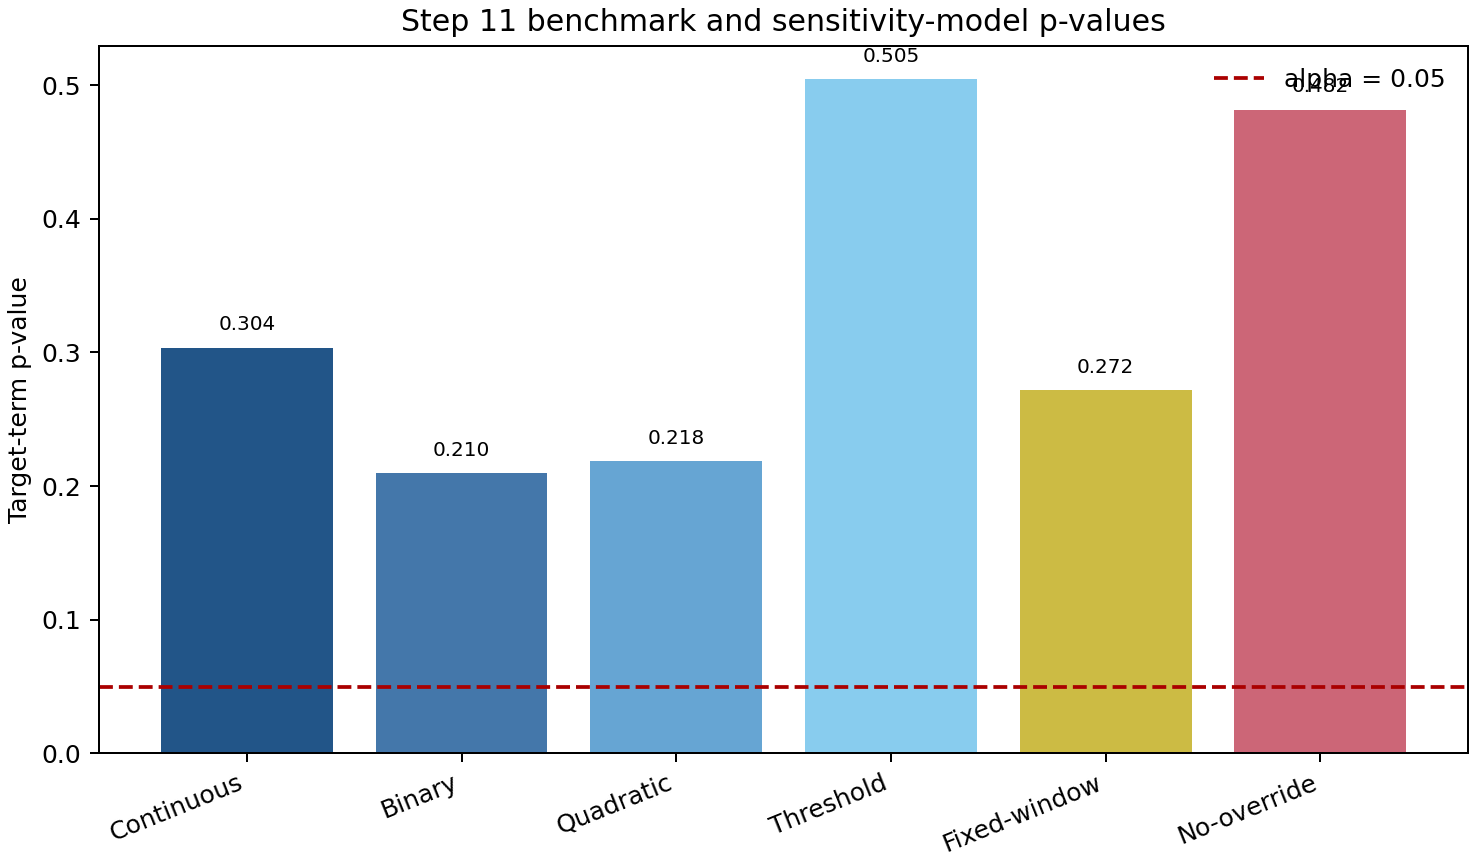
\includegraphics[width=0.48\linewidth]{../../figures/step11_visualization/sensitivity_pvalue_summary.png}
\caption{Leave-one-participant-out abstractness coefficients and the p-value summary across Step~11 benchmark/sensitivity models.}
\end{figure}
\begin{figure}[H]
\centering
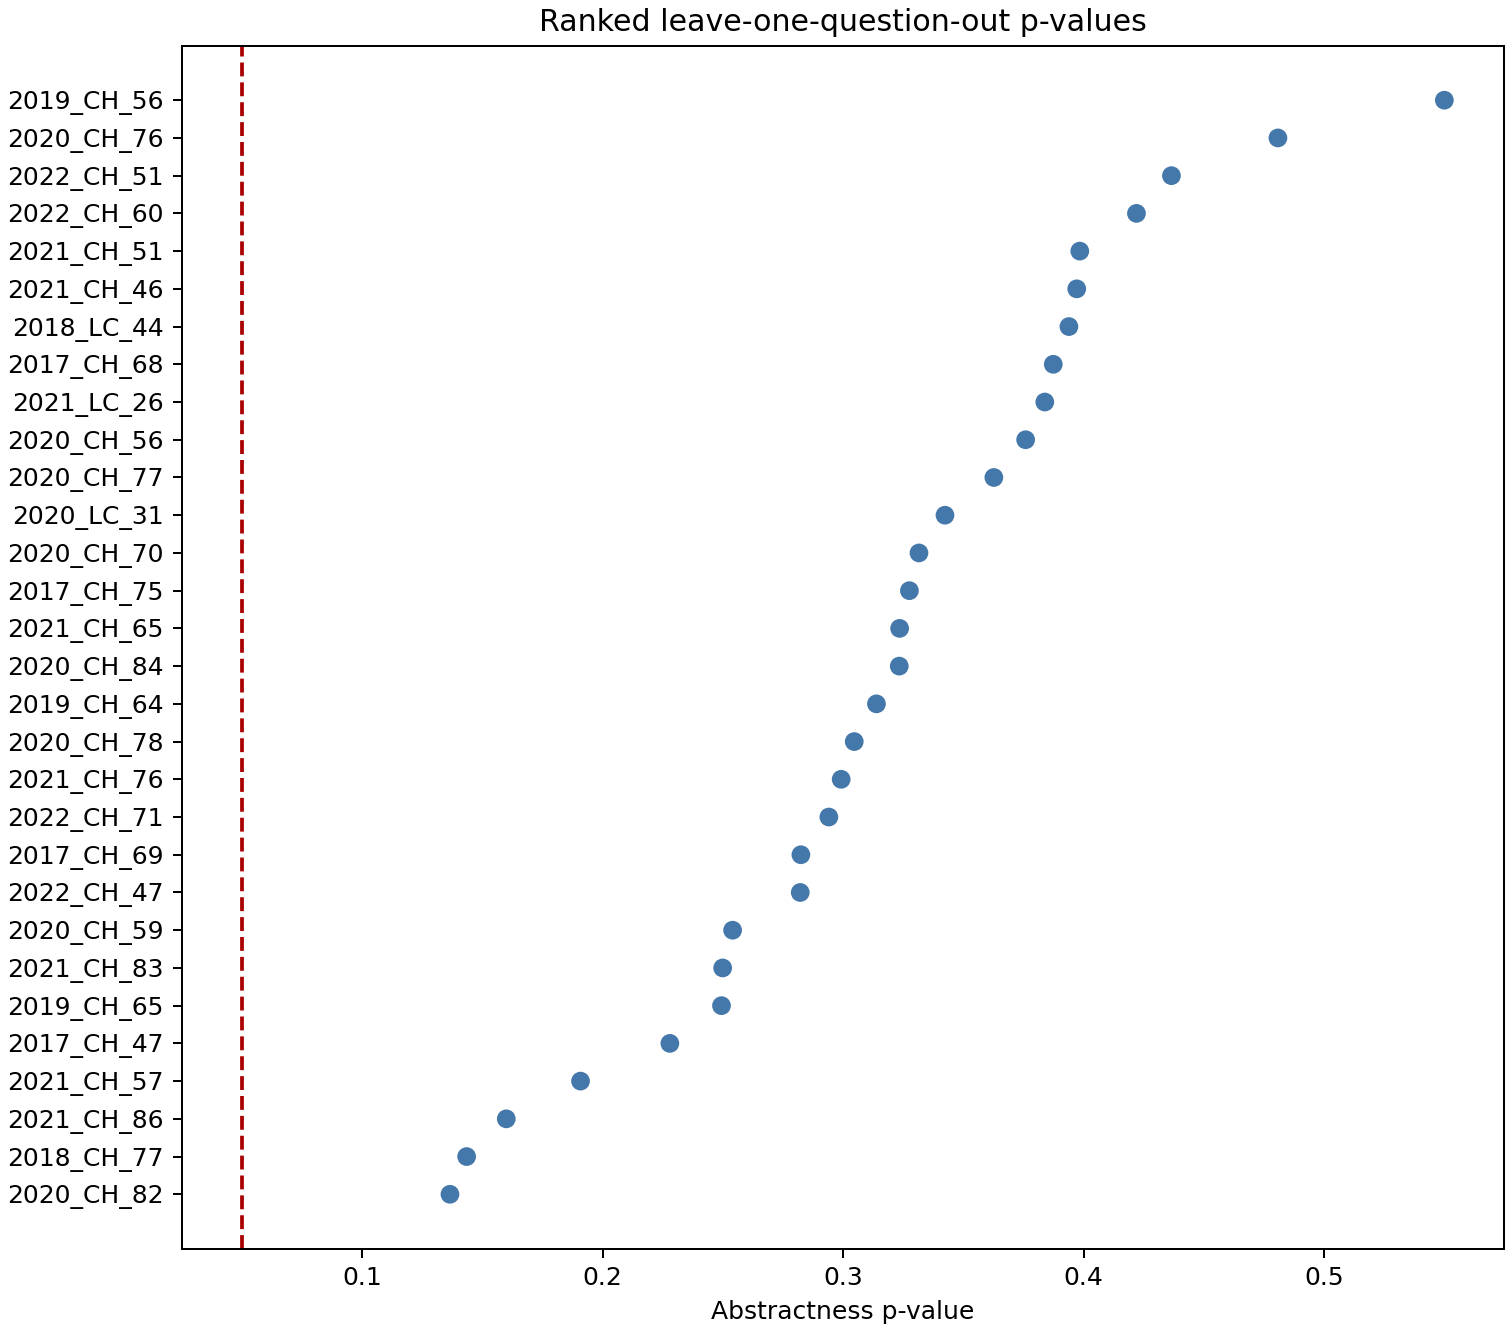
\includegraphics[width=0.48\linewidth]{../../figures/step11_visualization/leave_one_question_out_pvalues.png}
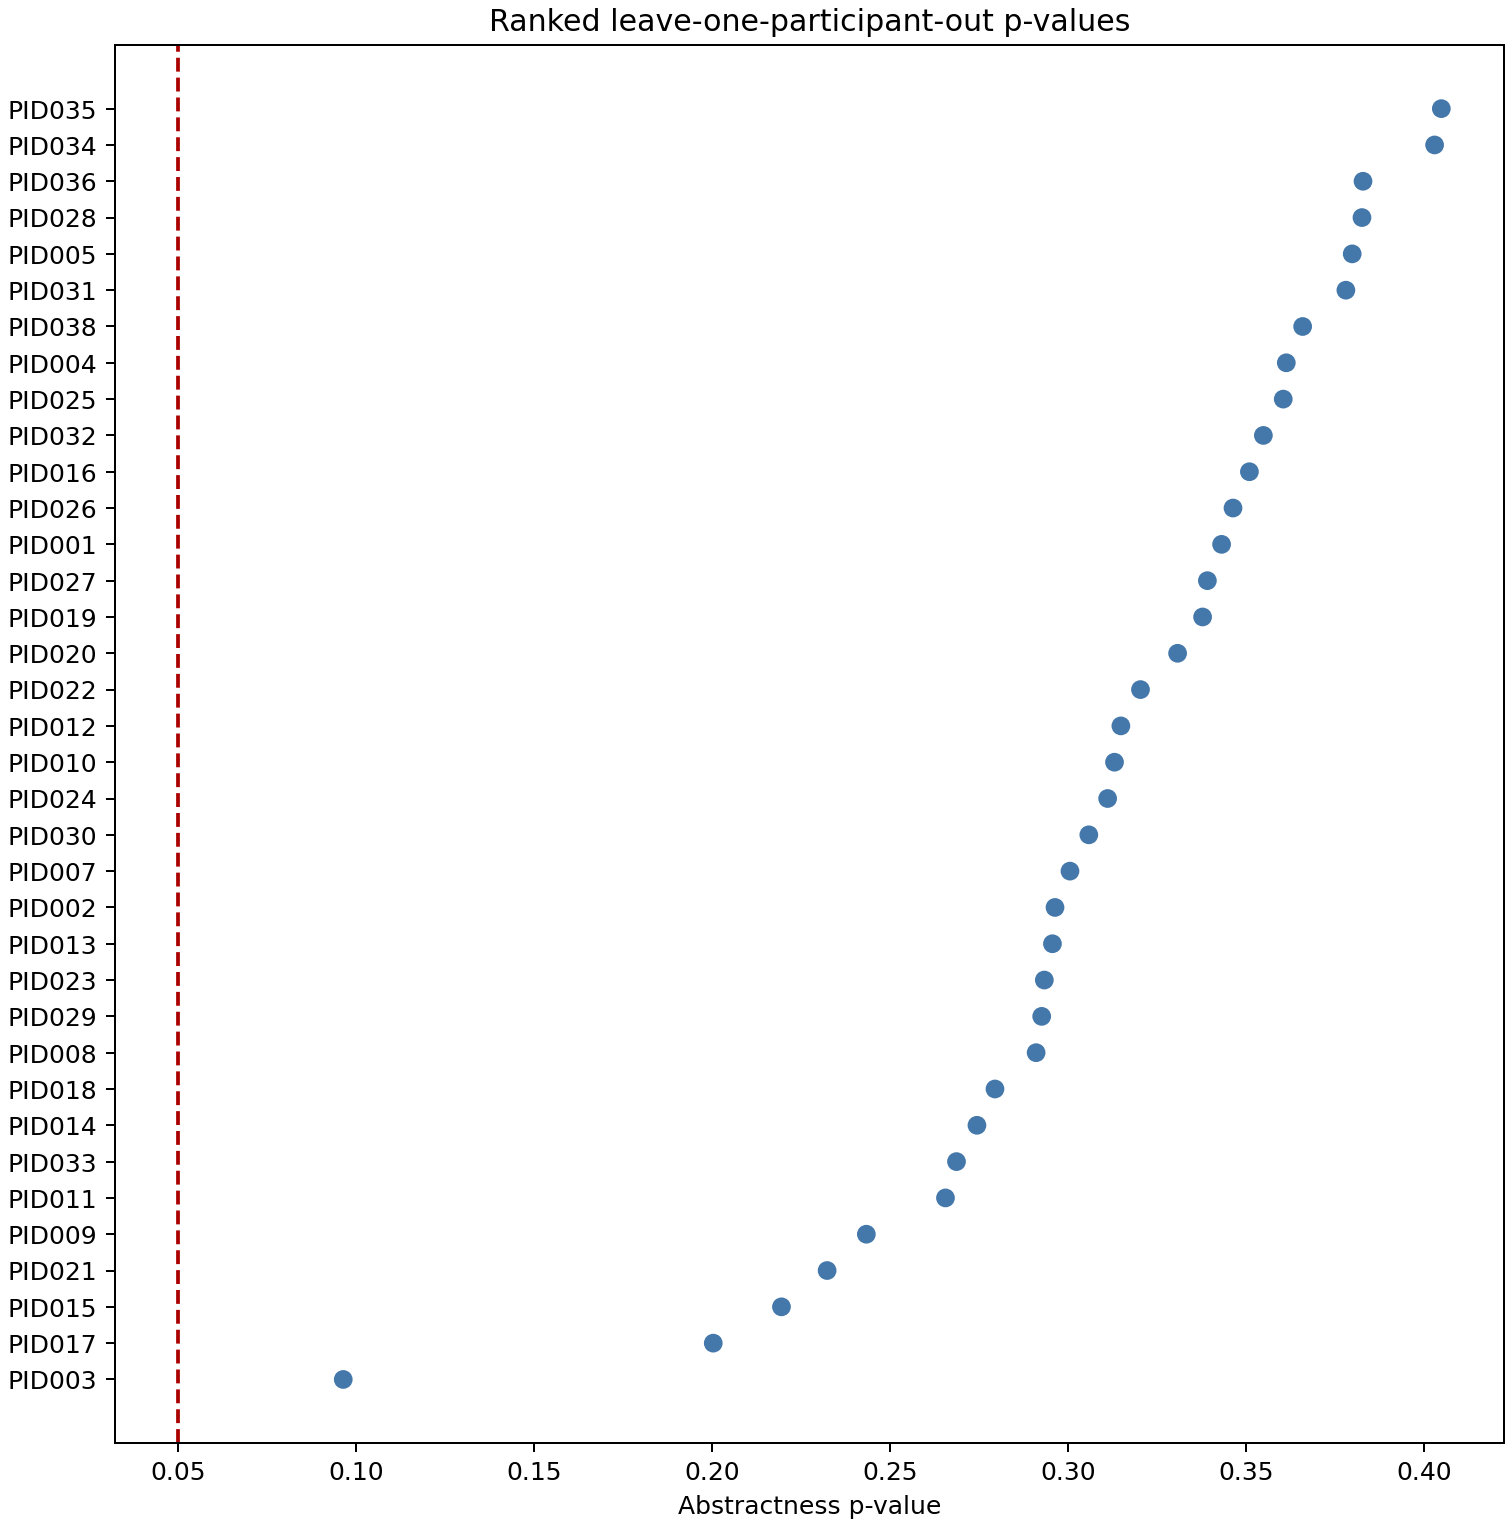
\includegraphics[width=0.48\linewidth]{../../figures/step11_visualization/leave_one_participant_out_pvalues.png}
\caption{Ranked p-values from the leave-one-question-out and leave-one-participant-out analyses. The red line marks alpha=0.05.}
\end{figure}
\end{document}
